% Options for packages loaded elsewhere
\PassOptionsToPackage{unicode}{hyperref}
\PassOptionsToPackage{hyphens}{url}
%
\documentclass[
]{article}
\usepackage{lmodern}
\usepackage{amssymb,amsmath}
\usepackage{ifxetex,ifluatex}
\ifnum 0\ifxetex 1\fi\ifluatex 1\fi=0 % if pdftex
  \usepackage[T1]{fontenc}
  \usepackage[utf8]{inputenc}
  \usepackage{textcomp} % provide euro and other symbols
\else % if luatex or xetex
  \usepackage{unicode-math}
  \defaultfontfeatures{Scale=MatchLowercase}
  \defaultfontfeatures[\rmfamily]{Ligatures=TeX,Scale=1}
\fi
% Use upquote if available, for straight quotes in verbatim environments
\IfFileExists{upquote.sty}{\usepackage{upquote}}{}
\IfFileExists{microtype.sty}{% use microtype if available
  \usepackage[]{microtype}
  \UseMicrotypeSet[protrusion]{basicmath} % disable protrusion for tt fonts
}{}
\makeatletter
\@ifundefined{KOMAClassName}{% if non-KOMA class
  \IfFileExists{parskip.sty}{%
    \usepackage{parskip}
  }{% else
    \setlength{\parindent}{0pt}
    \setlength{\parskip}{6pt plus 2pt minus 1pt}}
}{% if KOMA class
  \KOMAoptions{parskip=half}}
\makeatother
\usepackage{xcolor}
\IfFileExists{xurl.sty}{\usepackage{xurl}}{} % add URL line breaks if available
\IfFileExists{bookmark.sty}{\usepackage{bookmark}}{\usepackage{hyperref}}
\hypersetup{
  pdftitle={Reproducible Research: United Nations Voting Pattern: Bangladesh},
  pdfauthor={Abu Zafor Khairuzzaman},
  hidelinks,
  pdfcreator={LaTeX via pandoc}}
\urlstyle{same} % disable monospaced font for URLs
\usepackage[margin=1in]{geometry}
\usepackage{color}
\usepackage{fancyvrb}
\newcommand{\VerbBar}{|}
\newcommand{\VERB}{\Verb[commandchars=\\\{\}]}
\DefineVerbatimEnvironment{Highlighting}{Verbatim}{commandchars=\\\{\}}
% Add ',fontsize=\small' for more characters per line
\usepackage{framed}
\definecolor{shadecolor}{RGB}{248,248,248}
\newenvironment{Shaded}{\begin{snugshade}}{\end{snugshade}}
\newcommand{\AlertTok}[1]{\textcolor[rgb]{0.94,0.16,0.16}{#1}}
\newcommand{\AnnotationTok}[1]{\textcolor[rgb]{0.56,0.35,0.01}{\textbf{\textit{#1}}}}
\newcommand{\AttributeTok}[1]{\textcolor[rgb]{0.77,0.63,0.00}{#1}}
\newcommand{\BaseNTok}[1]{\textcolor[rgb]{0.00,0.00,0.81}{#1}}
\newcommand{\BuiltInTok}[1]{#1}
\newcommand{\CharTok}[1]{\textcolor[rgb]{0.31,0.60,0.02}{#1}}
\newcommand{\CommentTok}[1]{\textcolor[rgb]{0.56,0.35,0.01}{\textit{#1}}}
\newcommand{\CommentVarTok}[1]{\textcolor[rgb]{0.56,0.35,0.01}{\textbf{\textit{#1}}}}
\newcommand{\ConstantTok}[1]{\textcolor[rgb]{0.00,0.00,0.00}{#1}}
\newcommand{\ControlFlowTok}[1]{\textcolor[rgb]{0.13,0.29,0.53}{\textbf{#1}}}
\newcommand{\DataTypeTok}[1]{\textcolor[rgb]{0.13,0.29,0.53}{#1}}
\newcommand{\DecValTok}[1]{\textcolor[rgb]{0.00,0.00,0.81}{#1}}
\newcommand{\DocumentationTok}[1]{\textcolor[rgb]{0.56,0.35,0.01}{\textbf{\textit{#1}}}}
\newcommand{\ErrorTok}[1]{\textcolor[rgb]{0.64,0.00,0.00}{\textbf{#1}}}
\newcommand{\ExtensionTok}[1]{#1}
\newcommand{\FloatTok}[1]{\textcolor[rgb]{0.00,0.00,0.81}{#1}}
\newcommand{\FunctionTok}[1]{\textcolor[rgb]{0.00,0.00,0.00}{#1}}
\newcommand{\ImportTok}[1]{#1}
\newcommand{\InformationTok}[1]{\textcolor[rgb]{0.56,0.35,0.01}{\textbf{\textit{#1}}}}
\newcommand{\KeywordTok}[1]{\textcolor[rgb]{0.13,0.29,0.53}{\textbf{#1}}}
\newcommand{\NormalTok}[1]{#1}
\newcommand{\OperatorTok}[1]{\textcolor[rgb]{0.81,0.36,0.00}{\textbf{#1}}}
\newcommand{\OtherTok}[1]{\textcolor[rgb]{0.56,0.35,0.01}{#1}}
\newcommand{\PreprocessorTok}[1]{\textcolor[rgb]{0.56,0.35,0.01}{\textit{#1}}}
\newcommand{\RegionMarkerTok}[1]{#1}
\newcommand{\SpecialCharTok}[1]{\textcolor[rgb]{0.00,0.00,0.00}{#1}}
\newcommand{\SpecialStringTok}[1]{\textcolor[rgb]{0.31,0.60,0.02}{#1}}
\newcommand{\StringTok}[1]{\textcolor[rgb]{0.31,0.60,0.02}{#1}}
\newcommand{\VariableTok}[1]{\textcolor[rgb]{0.00,0.00,0.00}{#1}}
\newcommand{\VerbatimStringTok}[1]{\textcolor[rgb]{0.31,0.60,0.02}{#1}}
\newcommand{\WarningTok}[1]{\textcolor[rgb]{0.56,0.35,0.01}{\textbf{\textit{#1}}}}
\usepackage{graphicx,grffile}
\makeatletter
\def\maxwidth{\ifdim\Gin@nat@width>\linewidth\linewidth\else\Gin@nat@width\fi}
\def\maxheight{\ifdim\Gin@nat@height>\textheight\textheight\else\Gin@nat@height\fi}
\makeatother
% Scale images if necessary, so that they will not overflow the page
% margins by default, and it is still possible to overwrite the defaults
% using explicit options in \includegraphics[width, height, ...]{}
\setkeys{Gin}{width=\maxwidth,height=\maxheight,keepaspectratio}
% Set default figure placement to htbp
\makeatletter
\def\fps@figure{htbp}
\makeatother
\setlength{\emergencystretch}{3em} % prevent overfull lines
\providecommand{\tightlist}{%
  \setlength{\itemsep}{0pt}\setlength{\parskip}{0pt}}
\setcounter{secnumdepth}{-\maxdimen} % remove section numbering

\title{Reproducible Research: United Nations Voting Pattern: Bangladesh}
\author{Abu Zafor Khairuzzaman}
\date{}

\begin{document}
\maketitle

In this exploratory data analysis, we will explore the United nations
voting pattern, specially Bangladesh voting pattern. For this analysis
we will use two data set collected from datacamp repository:

\begin{enumerate}
\def\labelenumi{\arabic{enumi}.}
\tightlist
\item
  votes.rds
\item
  descriptions.rds (will add details later)
\end{enumerate}

\hypertarget{loading-the-data}{%
\subsection{Loading the data}\label{loading-the-data}}

\begin{Shaded}
\begin{Highlighting}[]
\NormalTok{fileUrl <-}\StringTok{ "http://dataverse.harvard.edu/api/access/datafile/:persistentId?persistentId=doi:10.7910/DVN/LEJUQZ/HAPPV6"}
\NormalTok{fileName <-}\StringTok{ "UNVotes.csv"}
\ControlFlowTok{if}\NormalTok{(}\KeywordTok{file.exists}\NormalTok{(}\KeywordTok{paste}\NormalTok{(}\StringTok{"data/"}\NormalTok{,fileName)))\{}
  \CommentTok{#download.file(fileUrl, destfile = "data/UNVotes.csv", method = "curl")}
\NormalTok{  dateDownloaded <-}\StringTok{ }\KeywordTok{date}\NormalTok{()}
\NormalTok{\}}

\NormalTok{votes <-}\StringTok{ }\KeywordTok{read.csv}\NormalTok{(}\StringTok{"data/UNVotes.csv"}\NormalTok{)}
\NormalTok{votes <-}\StringTok{ }\KeywordTok{as_tibble}\NormalTok{(votes)}
\KeywordTok{str}\NormalTok{(votes)}
\end{Highlighting}
\end{Shaded}

\begin{verbatim}
## tibble [1,216,585 x 26] (S3: tbl_df/tbl/data.frame)
##  $ rcid         : int [1:1216585] 3 3 3 3 3 3 3 3 3 3 ...
##  $ ccode        : int [1:1216585] 2 20 31 40 41 42 51 52 53 54 ...
##  $ member       : int [1:1216585] 1 1 NA 1 1 1 NA NA NA NA ...
##  $ vote         : int [1:1216585] 1 3 9 1 1 1 9 9 9 9 ...
##  $ Country      : Factor w/ 390 levels "AFG","AFGHANISTAN",..: 371 61 38 85 153 100 172 351 49 98 ...
##  $ Countryname  : Factor w/ 202 levels "Afghanistan",..: 190 33 12 43 76 52 87 180 15 51 ...
##  $ year         : int [1:1216585] 1946 1946 1946 1946 1946 1946 1946 1946 1946 1946 ...
##  $ session      : int [1:1216585] 1 1 1 1 1 1 1 1 1 1 ...
##  $ abstain      : int [1:1216585] 4 4 4 4 4 4 4 4 4 4 ...
##  $ yes          : int [1:1216585] 29 29 29 29 29 29 29 29 29 29 ...
##  $ no           : int [1:1216585] 18 18 18 18 18 18 18 18 18 18 ...
##  $ importantvote: int [1:1216585] 0 0 0 0 0 0 0 0 0 0 ...
##  $ date         : Factor w/ 864 levels "1946-01-01","1946-01-02",..: 1 1 1 1 1 1 1 1 1 1 ...
##  $ unres        : Factor w/ 5704 levels "","A/RES/71/102",..: 338 338 338 338 338 338 338 338 338 338 ...
##  $ amend        : int [1:1216585] 1 1 1 1 1 1 1 1 1 1 ...
##  $ para         : int [1:1216585] 0 0 0 0 0 0 0 0 0 0 ...
##  $ short        : Factor w/ 2022 levels "","?áINTERNATIONAL TRADE",..: 83 83 83 83 83 83 83 83 83 83 ...
##  $ descr        : Factor w/ 4558 levels "","0","10th anniversary of the adoption of the Declaration on the Preparation of Societies for Life in Peace",..: 2299 2299 2299 2299 2299 2299 2299 2299 2299 2299 ...
##  $ me           : int [1:1216585] 0 0 0 0 0 0 0 0 0 0 ...
##  $ nu           : int [1:1216585] 0 0 0 0 0 0 0 0 0 0 ...
##  $ di           : int [1:1216585] 0 0 0 0 0 0 0 0 0 0 ...
##  $ hr           : int [1:1216585] 0 0 0 0 0 0 0 0 0 0 ...
##  $ co           : int [1:1216585] 0 0 0 0 0 0 0 0 0 0 ...
##  $ ec           : int [1:1216585] 0 0 0 0 0 0 0 0 0 0 ...
##  $ ident        : int [1:1216585] 0 0 0 0 0 0 0 0 0 0 ...
##  $ resid        : int [1:1216585] 1001 1001 1001 1001 1001 1001 1001 1001 1001 1001 ...
\end{verbatim}

The vote column of the votes dataset represent the vote of country for a
particular issue. The number indicates as:

\begin{itemize}
\tightlist
\item
  1 = Yes
\item
  2 = Abstain
\item
  3 = No
\item
  8 = Not present
\item
  9 = Not a member
\end{itemize}

In our analysis we just consider first 3 type of votes, Yes, Abstain \&
No.~So in below step we will filter out the remaining.

\begin{Shaded}
\begin{Highlighting}[]
\NormalTok{votes <-}\StringTok{ }\NormalTok{votes }\OperatorTok
\StringTok{  }\KeywordTok{filter}\NormalTok{(vote }\OperatorTok{<=}\StringTok{ }\DecValTok{3}\NormalTok{)}

\KeywordTok{head}\NormalTok{(votes)}
\end{Highlighting}
\end{Shaded}

\begin{verbatim}
## # A tibble: 6 x 26
##    rcid ccode member  vote Country Countryname  year session abstain   yes    no
##   <int> <int>  <int> <int> <fct>   <fct>       <int>   <int>   <int> <int> <int>
## 1     3     2      1     1 USA     United Sta~  1946       1       4    29    18
## 2     3    20      1     3 CAN     Canada       1946       1       4    29    18
## 3     3    40      1     1 CUB     Cuba         1946       1       4    29    18
## 4     3    41      1     1 HTI     Haiti        1946       1       4    29    18
## 5     3    42      1     1 DOM     Dominican ~  1946       1       4    29    18
## 6     3    70      1     1 MEX     Mexico       1946       1       4    29    18
## # ... with 15 more variables: importantvote <int>, date <fct>, unres <fct>,
## #   amend <int>, para <int>, short <fct>, descr <fct>, me <int>, nu <int>,
## #   di <int>, hr <int>, co <int>, ec <int>, ident <int>, resid <int>
\end{verbatim}

\hypertarget{summarizing-votes}{%
\subsection{Summarizing votes}\label{summarizing-votes}}

In this section we will summarize the votes cast by Bangladesh and plot
the data to visualize.

\begin{Shaded}
\begin{Highlighting}[]
\NormalTok{votes_processed_bangladesh <-}\StringTok{ }\NormalTok{votes }\OperatorTok
\StringTok{  }\KeywordTok{filter}\NormalTok{(Countryname }\OperatorTok{==}\StringTok{ "Bangladesh"}\NormalTok{) }\OperatorTok
\StringTok{  }\KeywordTok{group_by}\NormalTok{(year) }\OperatorTok
\StringTok{  }\KeywordTok{summarize}\NormalTok{(}\DataTypeTok{total =} \KeywordTok{n}\NormalTok{(), }\DataTypeTok{percent_yes =} \KeywordTok{mean}\NormalTok{(vote }\OperatorTok{==}\StringTok{ }\DecValTok{1}\NormalTok{))}

\KeywordTok{ggplot}\NormalTok{(votes_processed_bangladesh, }\KeywordTok{aes}\NormalTok{(}\DataTypeTok{x =}\NormalTok{ year, }\DataTypeTok{y =}\NormalTok{ percent_yes)) }\OperatorTok{+}\StringTok{ }\KeywordTok{geom_line}\NormalTok{()}
\end{Highlighting}
\end{Shaded}

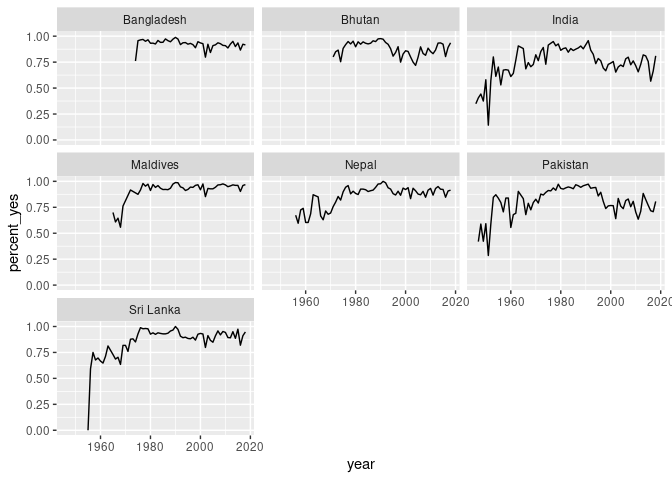
\includegraphics{UN_voting_files/figure-latex/unnamed-chunk-6-1.pdf}

From the line plot we can easily say that most of the time \textbf{Yes}
vote casting by Bangladesh over \textbf{85\%}.

Lets do some comparison with the South Asian countries.

\begin{Shaded}
\begin{Highlighting}[]
\NormalTok{countries <-}\StringTok{ }\KeywordTok{c}\NormalTok{(}\StringTok{"Bangladesh"}\NormalTok{, }\StringTok{"Bhutan"}\NormalTok{, }\StringTok{"India"}\NormalTok{, }\StringTok{"Maldives"}\NormalTok{, }\StringTok{"Nepal"}\NormalTok{, }\StringTok{"Pakistan"}\NormalTok{, }\StringTok{"Sri Lanka"}\NormalTok{)}
\NormalTok{votes_processed <-}\StringTok{ }\NormalTok{votes }\OperatorTok
\StringTok{  }\KeywordTok{filter}\NormalTok{(Countryname }\OperatorTok\StringTok{ }\NormalTok{countries) }\OperatorTok
\StringTok{  }\KeywordTok{group_by}\NormalTok{(Countryname, year) }\OperatorTok
\StringTok{  }\KeywordTok{summarize}\NormalTok{(}\DataTypeTok{total =} \KeywordTok{n}\NormalTok{(), }\DataTypeTok{percent_yes =} \KeywordTok{mean}\NormalTok{(vote }\OperatorTok{==}\StringTok{ }\DecValTok{1}\NormalTok{))}

\KeywordTok{ggplot}\NormalTok{(votes_processed, }\KeywordTok{aes}\NormalTok{(}\DataTypeTok{x =}\NormalTok{ year, }\DataTypeTok{y =}\NormalTok{ percent_yes)) }\OperatorTok{+}\StringTok{ }\KeywordTok{geom_line}\NormalTok{() }\OperatorTok{+}\StringTok{ }\KeywordTok{facet_wrap}\NormalTok{(}\OperatorTok{~}\StringTok{ }\NormalTok{Countryname)}
\end{Highlighting}
\end{Shaded}

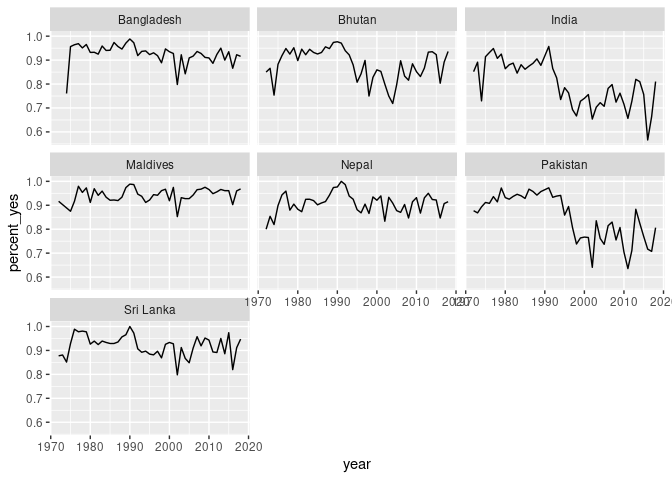
\includegraphics{UN_voting_files/figure-latex/unnamed-chunk-7-1.pdf}

From this comparison we can easily see that most of the time Bangladesh
cast positive vote (75\%-100\%). Lets do one more filter, since
Bangladesh born in 1971, we will consider the vote after 1971.

\begin{Shaded}
\begin{Highlighting}[]
\NormalTok{countries <-}\StringTok{ }\KeywordTok{c}\NormalTok{(}\StringTok{"Bangladesh"}\NormalTok{, }\StringTok{"Bhutan"}\NormalTok{, }\StringTok{"India"}\NormalTok{, }\StringTok{"Maldives"}\NormalTok{, }\StringTok{"Nepal"}\NormalTok{, }\StringTok{"Pakistan"}\NormalTok{, }\StringTok{"Sri Lanka"}\NormalTok{)}
\NormalTok{votes_processed <-}\StringTok{ }\NormalTok{votes }\OperatorTok
\StringTok{  }\KeywordTok{filter}\NormalTok{(Countryname }\OperatorTok\StringTok{ }\NormalTok{countries, year }\OperatorTok{>=}\StringTok{ }\DecValTok{1972}\NormalTok{) }\OperatorTok
\StringTok{  }\KeywordTok{group_by}\NormalTok{(Countryname, year) }\OperatorTok
\StringTok{  }\KeywordTok{summarize}\NormalTok{(}\DataTypeTok{total =} \KeywordTok{n}\NormalTok{(), }\DataTypeTok{percent_yes =} \KeywordTok{mean}\NormalTok{(vote }\OperatorTok{==}\StringTok{ }\DecValTok{1}\NormalTok{))}

\KeywordTok{ggplot}\NormalTok{(votes_processed, }\KeywordTok{aes}\NormalTok{(}\DataTypeTok{x =}\NormalTok{ year, }\DataTypeTok{y =}\NormalTok{ percent_yes)) }\OperatorTok{+}\StringTok{ }\KeywordTok{geom_line}\NormalTok{() }\OperatorTok{+}\StringTok{ }\KeywordTok{facet_wrap}\NormalTok{(}\OperatorTok{~}\StringTok{ }\NormalTok{Countryname)}
\end{Highlighting}
\end{Shaded}

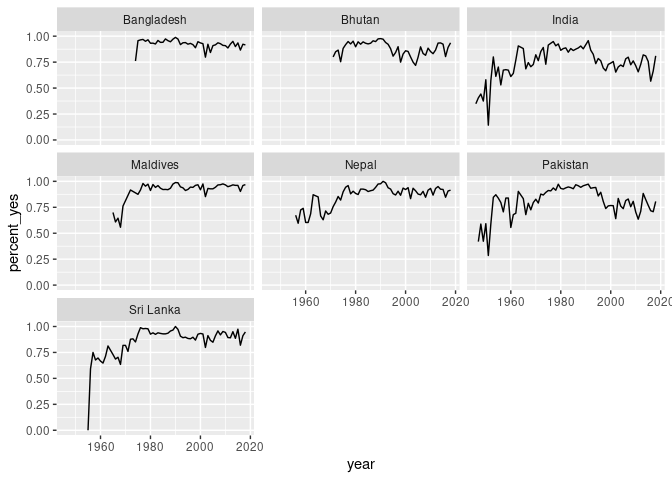
\includegraphics{UN_voting_files/figure-latex/unnamed-chunk-8-1.pdf}

In this time period (1972-2020), we can see that Bangladesh, Maldives,
Nepal \& Sri Lanka cast positive vote in between 80\%-100\%. They are
also consistent for casting positive vote.

\hypertarget{tidying-data}{%
\subsection{Tidying data}\label{tidying-data}}

In this section we will apply some operation to tidy the after and will
perform analysis on tidied data. We do not need all 26 columns in our
analysis so lets first subset the data with our required column.

\begin{Shaded}
\begin{Highlighting}[]
\NormalTok{votes_tidied <-}\StringTok{ }\NormalTok{votes }\OperatorTok
\StringTok{  }\KeywordTok{select}\NormalTok{(rcid}\OperatorTok{:}\NormalTok{session, unres,me}\OperatorTok{:}\NormalTok{ec)}
\end{Highlighting}
\end{Shaded}

There are 6 columns in the dataset that describe the topic of a
resolution,

\begin{itemize}
\tightlist
\item
  \textbf{me}: Palestinian conflict
\item
  \textbf{nu}: Nuclear weapons and nuclear material
\item
  \textbf{di}: Arms control and disarmament
\item
  \textbf{hr}: Human rights
\item
  \textbf{co}: Colonialism
\item
  \textbf{ec}: Economic development
\end{itemize}

Now, we will transform the data so that each row has one combination of
country-vote-topic so that we can analyze the graph by topic.

\begin{Shaded}
\begin{Highlighting}[]
\NormalTok{votes_tidied <-}\StringTok{ }\NormalTok{votes_tidied }\OperatorTok
\StringTok{  }\KeywordTok{gather}\NormalTok{(topic, has_topic, me}\OperatorTok{:}\NormalTok{ec) }\OperatorTok
\StringTok{  }\KeywordTok{filter}\NormalTok{(has_topic }\OperatorTok{==}\StringTok{ }\DecValTok{1}\NormalTok{)}
\end{Highlighting}
\end{Shaded}

It is difficult to interpret me, nu etc.. Lets re-code this abbreviation
with the actual name.

\begin{Shaded}
\begin{Highlighting}[]
\NormalTok{votes_tidied <-}\StringTok{ }\NormalTok{votes_tidied }\OperatorTok
\StringTok{  }\KeywordTok{mutate}\NormalTok{(}\DataTypeTok{topic =} \KeywordTok{recode}\NormalTok{(topic,}
                        \DataTypeTok{me =} \StringTok{"Palestinian conflict"}\NormalTok{,}
                        \DataTypeTok{nu =} \StringTok{"Nuclear weapons and nuclear material"}\NormalTok{,}
                        \DataTypeTok{di =} \StringTok{"Arms control and disarmament"}\NormalTok{,}
                        \DataTypeTok{hr =} \StringTok{"Human rights"}\NormalTok{,}
                        \DataTypeTok{co =} \StringTok{"Colonialism"}\NormalTok{,}
                        \DataTypeTok{ec =} \StringTok{"Economic development"}\NormalTok{))}

\NormalTok{by_country_year_topic <-}\StringTok{ }\NormalTok{votes_tidied }\OperatorTok
\StringTok{  }\KeywordTok{group_by}\NormalTok{(Countryname, year, topic) }\OperatorTok
\StringTok{  }\KeywordTok{summarize}\NormalTok{(}\DataTypeTok{total =} \KeywordTok{n}\NormalTok{(), }\DataTypeTok{percent_yes =} \KeywordTok{mean}\NormalTok{(vote }\OperatorTok{==}\StringTok{ }\DecValTok{1}\NormalTok{)) }\OperatorTok
\StringTok{  }\KeywordTok{ungroup}\NormalTok{()}
\end{Highlighting}
\end{Shaded}

Lets analyze topic wise vote for Bangladesh.

\begin{Shaded}
\begin{Highlighting}[]
\NormalTok{bd_by_country_year_topic <-}\StringTok{ }\NormalTok{by_country_year_topic }\OperatorTok
\StringTok{  }\KeywordTok{filter}\NormalTok{(Countryname }\OperatorTok{==}\StringTok{ "Bangladesh"}\NormalTok{)}

\KeywordTok{ggplot}\NormalTok{(bd_by_country_year_topic, }\KeywordTok{aes}\NormalTok{(}\DataTypeTok{x =}\NormalTok{ year, }\DataTypeTok{y =}\NormalTok{ percent_yes)) }\OperatorTok{+}\StringTok{ }\KeywordTok{geom_line}\NormalTok{() }\OperatorTok{+}\StringTok{ }
\StringTok{  }\KeywordTok{facet_wrap}\NormalTok{(}\OperatorTok{~}\StringTok{ }\NormalTok{topic)}
\end{Highlighting}
\end{Shaded}

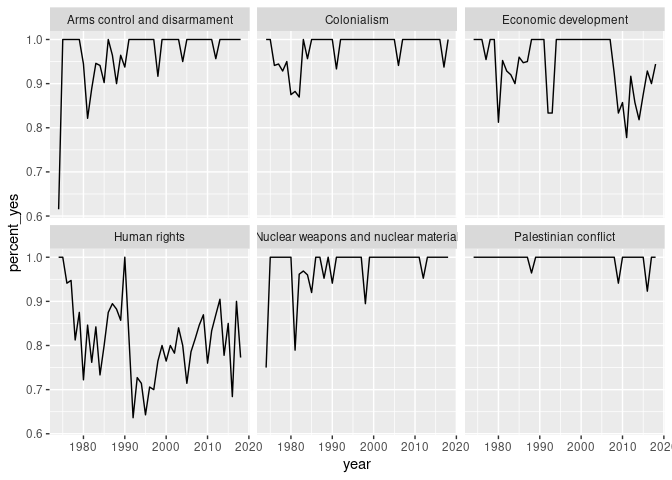
\includegraphics{UN_voting_files/figure-latex/unnamed-chunk-12-1.pdf} We
can see that for Human rights Bangladesh's votes has vary significantly
over time.

\end{document}
